\documentclass{report}
\usepackage{graphicx} % Required for inserting images
\usepackage{fancyhdr}
\usepackage{biblatex}
  \usepackage[french]{babel}
\usepackage{csquotes}
\usepackage[T1]{fontenc}
\usepackage[margin=3cm]{geometry}

\addbibresource{reference.bib} % reference location
\graphicspath{{./images/}} % image folder location

\title{Rapport \\ Alternance Banque de France - ESIEE Paris}
\author{Adrien PELFRESNE}
\date{
E3 Fillière informatique \\
Tuteurs : \\
ESIEE Paris : Abdelkrim Lahlou \\
Banque de France : Antoine Meheut \\ % mettre le rôle des tuteurs
Mars 2023
}

\begin{document}

\maketitle

Je tiens à remercier \emph{Antoine Meheut}, \emph{Sébastien Le Sausse} ainsi que toute l'équipe \emph{EXA} pour leur accueil chaleureux et leur soutien tout au long de ces premières périodes en entreprise. J'ai énormément appris, et cela n'aurait pas été possible sans une équipe accueillante et toujours prête à répondre à mes questions.

Je souhaite également remercier la \emph{Banque de France} pour m'avoir donné l'opportunité de réaliser mon alternance.
Enfin, je remercie \emph{ESIEE Paris} pour m'avoir donné les moyens d'apprendre et de me former. L'enseignement de haute qualité, l'encadrement et les opportunités offertes par l'école ont été essentiels pour me permettre d'acquérir les compétences techniques et les connaissances théoriques nécessaires au bon déroulement de mon alternance.
% tant sur la méthode que techniquement

\tableofcontents

\chapter{Présentation de la Banque De France}
Mon organisme d'accueil, la Banque De France, est une institution indispensable au fonctionnement de l'économie française. Elle agit dans de nombreux domaines d'activités et est l'interlocuteur de la coopération économique européenne.

\section{Missions}
La Banque de France est garante de trois missions principales : la stratégie monétaire, la stabilité financière et les services à l'économie.
\begin{itemize}
    \item \textit{Stratégie monétaire} : Elle est responsable de la mise en œuvre de la politique monétaire de la zone euro, en collaboration avec la \textbf{BCE} (Banque centrale européenne). Elle contribue à maintenir la stabilité des prix et à soutenir la croissance économique en contrôlant la quantité de monnaie en circulation dans l'économie. La Banque de France fixe également les taux d'intérêt directeurs pour les opérations de refinancement et veille à ce que les banques respectent les exigences de réserves obligatoires.
    \item \textit{Stabilité financière} : La Banque de France joue un rôle important dans la préservation de la stabilité financière en surveillant et en réglementant les institutions financières, notamment les banques, les compagnies d'assurance et les entreprises d'investissement. Elle est chargée de surveiller les risques systémiques dans le système financier français et de mettre en place des mécanismes de résolution en cas de crise financière. Dans ce contexte, la Banque de France participe aux travaux internationaux de réglementation financière.
    \item \textit{Services à l'économie} : Elle fournit des services à l'économie française, en gérant les paiements de l'État et en facilitant les opérations de change pour les entreprises et les particuliers. Elle est responsable de la production et de la distribution de billets de banque en France, ainsi que de la surveillance de la circulation des billets contrefaits. Enfin, elle effectue des enquêtes économiques et financières pour fournir des informations utiles aux décideurs politiques et aux entreprises.
\end{itemize}

\section{Historique}
La Banque de France a été créée en 1800 par Napoléon Bonaparte pour renforcer le système financier du pays et aider à financer les guerres napoléoniennes. Pendant la majeure partie de son histoire, la Banque de France a été une institution centrale puissante, responsable de la politique monétaire et de la réglementation bancaire en France.
Au fil du temps, elle a également pris en charge d'autres fonctions importantes, telles que la gestion des réserves de change et la supervision de l'émission de billets de banque. Elle a été un acteur clé dans la création de l'euro en tant que monnaie unique de l'Union européenne.
Au cours du XXe siècle, la Banque de France a connu des périodes de réforme et de modernisation, notamment après la Seconde Guerre mondiale, lorsque la France a adopté un système de taux de change flottants et a introduit une nouvelle monnaie, le franc français.
Aujourd'hui, elle est toujours une institution centrale indépendante, qui opérant dans un cadre réglementaire strict et jouant un rôle clé dans la stabilité financière de la France et de l'Union européenne.


\section{Cœurs de métier}
Les activités de la BDF (Banque de France) sont très diverses. On peut répartir les activités en 10 grandes catégories de métiers \cite{BdfLesMetiers}

\subsection{Fabrication de billets}
La Banque de France a une activité industrielle de fabrication des billets. Elle participe à l'impression d'une partie des billets en euros en vertu d'accords européens et fabrique également des billets pour des banques centrales étrangères.

\subsection{Gestion de la monnaie fiduciaire}
La Banque de France assure via son réseau de caisses la mise en circulation des pièces et billets en euros sur l’ensemble du territoire métropolitain et le recyclage d’une part significative de ces billets.
Elle assure le contrôle d'une partie de l'activité fiduciaire exercé par les banques ou transporteur de fond.

\subsection{Opérations}
La Banque de France a pour mission d'assumer quatre responsabilités principales qui sont étroitement liées à la Banque Centrale Européenne. Ces responsabilités comprennent la réalisation des opérations de marché et la mise en œuvre de la politique monétaire, la surveillance des systèmes de paiement et des infrastructures de marché, la prestation de services bancaires aux clients institutionnels tels que le Trésor public et les établissements financiers, ainsi que la coordination de la stabilité financière.

\subsection{Statistiques, recherches et relations internationales}
La Banque de France a pour rôle de produire et diffuser des statistiques, des indicateurs et des études économiques, monétaires et financières. Ces informations sont utilisées pour préparer et expliquer les décisions de politique monétaire. En outre, la Banque de France participe aux travaux des principales organisations économiques et financières internationales telles que le \textbf{FMI} (Fonds Monétaire International), la \textbf{BRI} (Banque des règlements internationaux) et la \textbf{BCE} (Banque Centrale Européenne), ainsi qu'aux instances internationales comme le \textbf{G8} ou le \textbf{forum de stabilité financière}.

\subsection{Supervision prudentielle}
La Banque de France agit en tant que superviseur des établissements bancaires, des compagnies d'assurance et des mutuelles. Pour le compte de \textbf{l'ACPR} (Autorité de contrôle prudentiel et de résolution), elle vérifie que ces institutions respectent des règles de prudence visant à accroître la stabilité financière, à renforcer la sécurité des consommateurs et à faire entendre la voix de la France dans les instances européennes et internationales.

\subsection{Présence de place}
La Banque de France offre divers services dans les régions, qui profitent aux particuliers, aux collectivités publiques et aux banques. Ces services comprennent la gestion du surendettement des ménages, la collecte, l'analyse et la mise à disposition d'informations sur les entreprises non financières, ainsi que la gestion et l'animation du réseau de succursales.


\subsection{Gestion, logistique et communication}
Pour que la Banque de France puisse exercer ses activités, plusieurs fonctions de support sont nécessaires. Chacune de ces fonctions joue un rôle important dans le bon fonctionnement de l'institution :
\begin{itemize}
    \item La programmation budgétaire, la comptabilité et le contrôle de gestion
    \item La gestion de l'immobilier, la sécurité/sûreté et la logistique
    \item Les achats
    \item La communication.
\end{itemize}

\subsection{Ressources humaines}
La Banque de France soutient ses employés tout au long de leur carrière en encourageant la promotion interne et la mobilité. Elle renforce également sa réputation d'employeur de choix pour attirer des talents, et développe les compétences de ses employés grâce à la formation et à la gestion de carrière.

\subsection{Système d'informations}
La  \textbf{DGSI} (Direction Générale du Système d'Information) garantit le bon fonctionnement des activités de la Banque grâce à des services informatiques de qualité.
Elle joue un rôle clé dans les projets informatiques au niveau de l'Eurosystème et du \textbf{SEBC} (système européen des banques centrales).
La DGSI est également très impliquée dans la transformation numérique et est à la pointe de l'innovation organisationnelle et informatique.
Nous étudierons plus tard en détail la structure de la DGSI, étant la direction générale dans laquelle je travaille.

\subsection{Contrôle et préventions des risques}
Le service d'Audit interne évalue les processus de gestion, de maîtrise des risques et de contrôle interne de la Banque de France grâce aux missions menées par l'Inspection Générale dans les services centraux et le réseau de succursales. Le dispositif de gestion des risques opérationnels de la Banque de France est reconnu comme étant l'un des meilleurs du SEBC.

La direction de la Prévention des risques participe à divers groupes de travail internationaux pour maintenir ce dispositif au niveau des meilleures pratiques internationales.

En conclusion, la Banque de France est une institution financière majeure et la banque centrale française qui fait partie de l'Eurosystem. Elle est responsable de la stratégie monétaire, la stabilité financière et les services à l'économie. Ces activités sont très diverses. 

\section{Organigramme}
Nous allons, dans une première partie, aborder la structure générale de la \textbf{DGSI} (Direction générale du système d'information), en essayant de comprendre le rôle de chaque direction, cette description restera générale. Puis dans un second temps, nous étudierons plus en détail la structure de la \textbf{DISCO} (Direction des services communs), de \textbf{SIEDEV} (service d'industrialisation et d'expertise au développement) et enfin \textbf{d'EXA} (Expertise applicative)

\subsection{Générale}
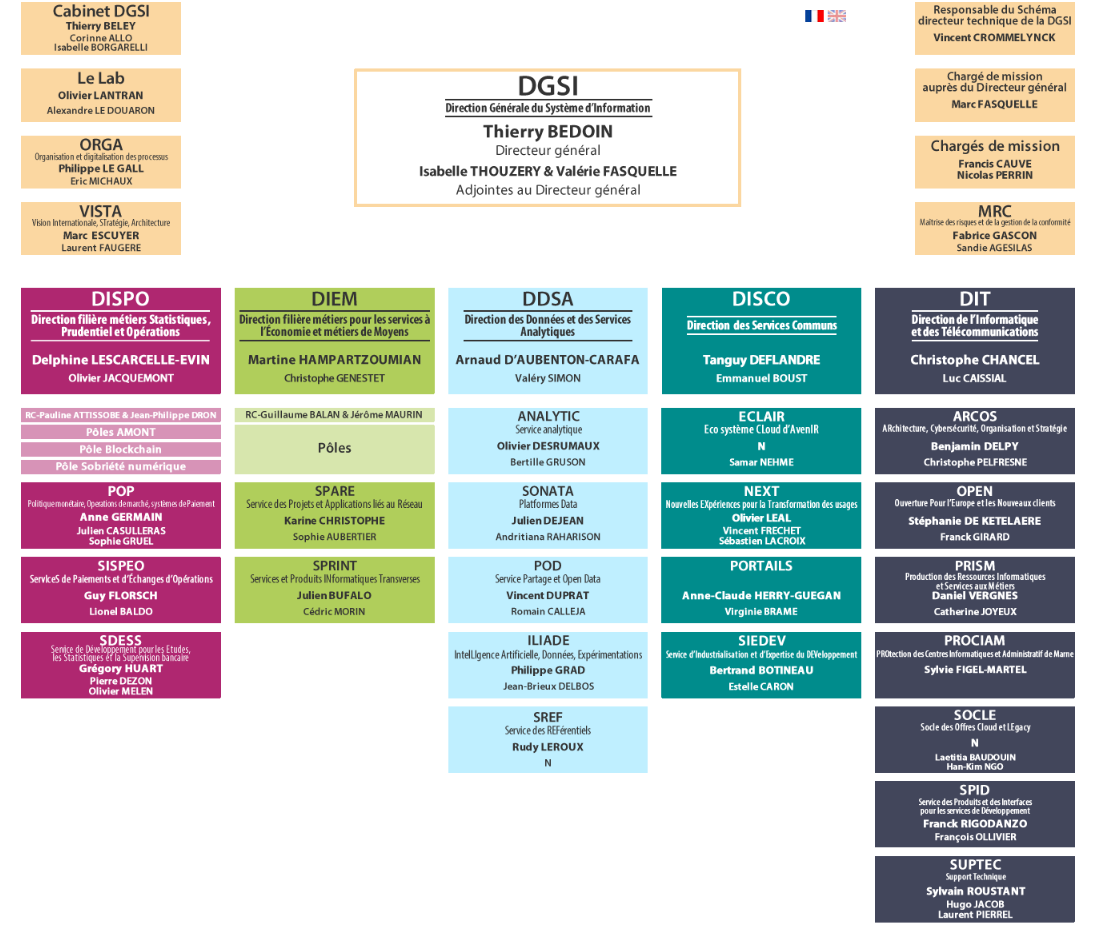
\includegraphics[scale=0.55]{ORGA}
Une direction générale, comme la DGSI, est divisé en plusieurs directions. on cite \textbf{DISPO} (direction filière métiers statistiques, prudentiel et opérations), \textbf{DIEM} (Direction filière métiers pour les services à l'économie et métiers de moyen), la \textbf{DDSA} (Direction des Données et des services Analytiques), la \textbf{DIT} Direction de l'informatique et des télécommunications, et enfin DISCO : ma direction.
DISCO est chargé d'assurer la fourniture de services communs, performants et sécurisés, internes ou externes. ses missions principales sont les suivantes :\\
\begin{itemize}
    \item Doter l'ensemble des collaborateurs d'un environnement de travail répondant aux meilleurs standards de sécurité, facilitant les nouveaux modes de travail, améliorant la transversalité avec des interlocuteurs internes comme externes, et allégeant la charge mentale.
    \item Fournir une offre cloud interne et externes adaptées aux besoins actuels et futurs de la Banque de France.
    \item Permettre l'adaptation de nos applications pour tendre vers une migration et un déploiement continue.
    \item Mettre à disposition une offre de portails standardisée avec un SI plus interopérable avec notamment l'usage des \textbf{API} (application programming interface).
\end{itemize}
Son organisation s'appuie sur 4 services.
\textbf{NEXT} (nouvelle expérience pour la transformation des usages) ayant pour objectif l'amélioration de l'expérience utilisateur par une vision globale et cohérente des solutions techniques et des services associés a l'environnement de travail digital, il supervise la gestion et de l'évolution de l'environnement de travail des utilisateurs, du choix des terminaux jusqu'aux outils collaboratifs.
\textbf{ECLAIR} (Eco-système cloud d'avenir) en charge du développement et de la fourniture des offres de services cloud.
\textbf{PORTAILS} (sans acronyme connu) responsable des composants communs des portails de la banque, (site institutionnel, mais aussi intranets).
SIEDEV prend en charge l'industrialisation du processus de développement d'applications ainsi que des outillages projets. Il met à disposition les expertises et gère-les outils logiciels et les plateformes permettant d'assurer la qualité et la sécurité du code, sa conformité aux différentes normes et règles en vigueur, et de déployer de manière la plus automatisée possible les applications sur les différents environnements jusqu'à leur mise en production.

Nous incluons ci-dessous l'organigramme de SIEDEV :

\begin{center}
   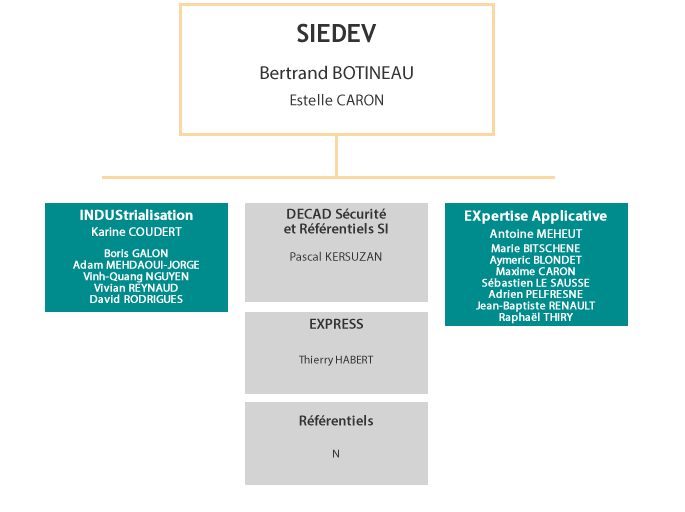
\includegraphics[scale=0.70]{SIEDEV} 
\end{center}

Le pôle dans lequel je travaille est EXA. c'est une cellule d'expertise et d'accompagnement de toutes les équipes de développements informatiques. EXA est garant de la définition et du respect des lignes de développement, et a aussi pour mission d'accompagner les CPI/DPI (Chef de Projet Informatique, Directeur de Projet Informatique), et de promouvoir les bonnes pratiques auprès de tous les acteurs de la Banque de France. EXA peut intervenir en support à un projet ou une application sous différentes formes. les principales sont : répondre à un ticket support JIRA, intervention d'un Techlead à temps plein ou partiel, participation direct des équipes à un projet ou un programme. EXA se charge aussi du maintien de la charte graphique de la BDF et propose des projets \textit{starter kits}, contenant les bonnes pratiques de sécurité et de développement.

\chapter{Travail réalisé}
\section{Contexte}
En intégrant EXA, l'équipe en charge de la sécurité applicative et des bonnes normes de développement à la banque de France,

% parler des langages dans exa, du type de travail que j'ai réalisé, du contexte dans lequel celui ci a été réalisé : agile, ci cr etc..

\section{Les objectifs à atteindre}

\section{Le cadre de travail : équipe de travail, interlocuteurs, collaborateurs}

\section{Les techniques et systèmes que vous avez dû découvrir}
J'ai des découverts de nombreux outils et techniques, dont je vais parer ici, une grande partie de ces outils n'est pas spécifique à la banque de France, mais utilisé dans beaucoup d'entreprise possédant un pôle de développement logiciels/web.

\section{Méthodes agiles}
% parler de la méthodologie agile qu'on utilise a la banque (demain demander a sébastien pour être sur que je ne me trompe pas sur laquelle on utilise)

\subsection{Gestion des sources}
\textit{Git} \cite{AboutGit} est un système de contrôle de version, utilisé pour suivre les changements apportés à des fichiers et des dossiers au fil du temps. Il permet aux utilisateurs de collaborer efficacement sur des projets, en facilitant la gestion des modifications et des versions. 
C'est un système distribué et multibranches. Chaque développeur peut travailler sur sa propre branche de code, indépendamment des autres développeurs. Chaque branche peut contenir des modifications uniques et séparées, sans affecter les autres branches. Cela permet aux développeurs de travailler de manière plus efficace et collaborative sur des projets de grande envergure. 
\textit{Git} permet aux développeurs d'expérimenter de nouvelles fonctionnalités ou de nouveaux changements sans affecter la branche principale ou le code en production. Ils peuvent créer une nouvelle branche, tester leurs modifications et si tout fonctionne correctement, ils peuvent ensuite fusionner leurs modifications dans la branche principale. l'utilisation de \textit{Git} permet à une entreprise de gérer les modifications de code de manière plus efficace et collaborative, ce qui se traduit par une meilleure qualité de code et des projets plus solides.
\begin{figure}
    \centering
    
\includegraphics[scale=0.08]{images/1280px-Git-logo.svg.png}
    \caption{logo de git}
    \label{fig:git}
\end{figure}

\textit{GitLab} est une plateforme de gestion de projets qui utilise \textit{Git} comme système de contrôle de version. \textit{GitLab} fournit une interface web pour gérer les référentiels \textit{Git}, ainsi que des fonctionnalités pour le suivi des problèmes, la gestion des projets, la planification agile et la collaboration en équipe.

\begin{figure}
    \centering
    
\includegraphics[scale=0.04]{images/Gitlab-Logo.png}
    \caption{logo de gitlab}
    \label{fig:gitlab}
\end{figure}

 \textit{Git} et \textit{GitLab} sont utilisés pour gérer les sources de tous les projets informatiques de la Banque de France.    
Cela n'a pas été facile pour moi de m'adapter à ce nouveau mode de gestion de source, bien qu'aillant utilisé ces technologies auparavant. Je n'avais jamais utilisé la fonctionnalité multibranches, n'en ayant pas les besoins.
Pour utiliser au mieux ces deux outils, quelque connaissance théorique et pratique sont nécessaires. Notamment la méthode \textit{Gitflow} \cite{Gitflow} qui codifie l'usage des branches et l'ajout de fonctionnalité.
Elle est conçue pour gérer efficacement les branches et les versions du logiciel. Nous allons voir comment \textit{gitflow} scinde les différentes branches et quelle sont leurs utilités. 
\begin{itemize}
    \item La branche \textit{master} ou \textit{main}: c'est la branche principale de développement qui contient le code de production stable. Elle est unique.
    \item La branche  \textit{develop} : c'est la branche de développement actuelle qui contient les dernières fonctionnalités et modifications qui ne sont pas encore en production. Elle est unique.
    \item Les branches \textit{features} : sont des branches créées à partir de la branche \textit{develop} pour ajouter une nouvelle fonctionnalité ou résoudre un problème spécifique. une branche \textit{feature} est fusionnée dans la branche \textit{develop} une fois la fonctionnalité fonctionnelles et testées, on compte autant de branches \textit{features} que de nouvelles fonctionnalités à ajouter.
    \item Les branches \textit{release} : sont créées à partir de la branche develop pour préparer une nouvelle version de production. Elles contiennent les derniers correctifs de bugs et les modifications de dernière minute. Elles sont fusionnées dans la branche master et develop une fois qu'elles sont terminées.
    \item Les branches \textit{hotfix} : sont des branches créées à partir de la branche \textit{master} pour résoudre rapidement des problèmes critiques de production. une branche  \textit{hotfix} est fusionné dans master et dans develop une fois que le problème a été corrigé. Ces branches \textit{hotfix} permettent de corriger un problème bloquant sans attendre une itération de release de l'application.
\end{itemize}

La méthodologie Gitflow permet de maintenir une structure de branche claire et organisée, cela la collaboration entre les membres de l'équipe et la gestion des versions du logiciel. Elle assure la qualité du code en permettant aux développeurs de travailler sur des branches de fonctionnalités et de corrections de bugs séparément.

\subsection{Pipeline et intégration continue}
L'intégration continue (CI) est une pratique de développement de logiciels consistant à fusionner régulièrement les modifications apportées au code dans la branche \textit{develop} et \textit{master}, afin de détecter et de résoudre rapidement les conflits d'intégration, en effet, plus les fusions sont effectuées souvent, moins il y a de conflits de fusions à gérer. En pratique, cela implique l'utilisation d'outils automatisés pour construire, tester et déployer des applications lorsque des changements aux branches principales sont effectués.

Un pipeline de CI/CD (intégration continue et déploiement continu) est un processus automatisé qui permet de gérer le cycle de vie d'une application, depuis la construction jusqu'à la livraison en production. Le pipeline est composé de plusieurs étapes, telles que la compilation, les tests unitaires, les tests d'intégration, la validation de la qualité du code, la construction d'artefacts et le déploiement.

En utilisant un pipeline de CI/CD, les développeurs peuvent accélérer la livraison de nouvelles fonctionnalités, améliorer la qualité du code et réduire les risques liés aux déploiements. Les équipes de développement peuvent ainsi garantir que les modifications du code sont testées et validées avant d'être intégrées dans la branche principale, et que les nouvelles fonctionnalités sont livrées en production de manière fiable et cohérente.

en pratique, cela se fait avec un pipeline Jenkins, 

\subsection{Gestion des demandes}
% parler de jira

\subsection{Cycle de vie d'une demande}
% expliquer les différentes étapes d'une demande, du ticket jira, jusquau merge de la branche de fix dans develop et de la release contenant la modification

\subsection{Documentation}
% parler de confluence

\section{Le travail effectué}

\section{Les difficultés techniques rencontrées}

\section{Les initiatives personnelles}

\section{L’état d’avancement actuel et les ouvertures éventuelles}
 
\printbibliography
\end{document}